\subsection{Обзор существующих аналогов}
\label{sec:analysis:analogues}

Для решения задач управления временем, задачами и контактами могут использоваться различные средства. Рассмотрим каждую из задач в\linebreakотдельности.
\newline
\subsubsection{} Управление временем и расписаниями
\label{sec:analysis:analogues:schedules}

Для участников учебного процесса управление временем заключается в следовании расписанию, составляемое деканатами или диспетчерской службой университетов. Еще тридцать лет назад расписание представляло собой таблицу на огромном листе бумаги, которую составляли вручную и вывешивали на доске объявлений. Чтобы узнать, какое занятие будет следующим, приходилось или заранее переписывать своё расписание всем студентам, или каждый раз идти к доске объявлений (что имеет свои преимущества, так как тогда есть возможность узнать обо всех изменениях в расписании).

С течением времени от ручного заполнения перешли к составлению электронных таблиц в специальных программных средствах. Тем не менее, облегчено было только составление расписания, а не пользование им: электронные таблицы печатались и по-прежнему вывешивались около деканатов. Потребовалось еще несколько лет и прогресс в развитии информационных технологий, чтобы студенты и преподаватели получили возможность получения расписания через сеть интернет без необходимости посещения университета.

В настоящее время на постсоветском пространстве существует огромное число высших учебных заведений. Некоторое время назад процессы, происходящие в таких учреждениях не были оцифрованы и автоматизированы вовсе. Лишь недавно начали появляться информационные системы, решающие те или иные задачи. Однако, каждый ВУЗ занимается этой проблемой самостоятельно и решает ее, насколько хватает квалифицированных специалистов, ресурсов и, самое главное, желания внедрять что-то инновационное со стороны руководства и участников учебного процесса этих ВУЗов.

Универсальной шкалы, позволяющей оценить удобство следования по всем деятельностям учебного процесса в разных ВУЗах, нет. Однако, можно попытаться это оценить по некоторым вторичным признакам, таким как, например, соответствие сайта ВУЗа современным представлениям об удобстве пользования (можно легко отличить сайты, сделанные за последние несколько лет, от сайтов, сделанных более десяти лет назад: со временем меняются и представления об удобстве пользования, и технологии, позволяющие его достичь), отзывах тех людей, которые участвуют в процессе обучения (то есть студентов, преподавателей) и некоторым другим. Рассмотрим возможности, предоставляемые информационными системами различных белорусских ВУЗов по состоянию на апрель 2017 года.

Белорусский государственный университет информатики
как ведущий специализированный университет в области информационных технологий на постсоветском пространстве обладает достаточным числом квалифицированных специалистов (поскольку обучает их), чтобы автоматизировать многие части учебного процесса. Для пользования предоставляется система расписания: занятий и экзаменов для студентов и преподавателей, причём предоставляется возможность не только просматривать расписание, находясь на сайте (пример расписания приведен на рисунке \ref{fig:analysis:analogues:bsuir}), но реализован API для получения актуальных данных о преподавателях, группах и расписании для них в формате XML. Помимо этого, наиболее близкий к информационным технологиям факультет компьютерных систем и сетей (КСиС) имеет в своём распоряжении портал факультета, на котором присутствует актуальная информация о событиях, происходящих на факультете, куда выкладываются расписания учебного процесса, списки групп, рейтинговые списки. Однако, по-прежнему существует и ряд проблем. Кроме факультета КСиС, своих порталов не имеет ни один из других факультетов, поэтому вся коммуникация со студентами может происходить только очно, а некоторые неформальные виды коммуникации -- через группы факультетов в социальных сетях. Кафедры не имеют удобной для студентов доски объявлений (строго говоря, такие доски есть, но она находится настолько глубоко внутри сайта университета, что большая часть студентов о ней и не знает). Для того, чтобы внести любое малейшее изменение в расписание, преподавателю нужно обращаться в диспетчерскую службу: нет возможности сделать это автоматически. Но несмотря на все недостатки, БГУИР все равно обгоняет многие ВУЗы по степени информатизации и автоматизации учебного процесса.

\begin{figure}
	\centering
	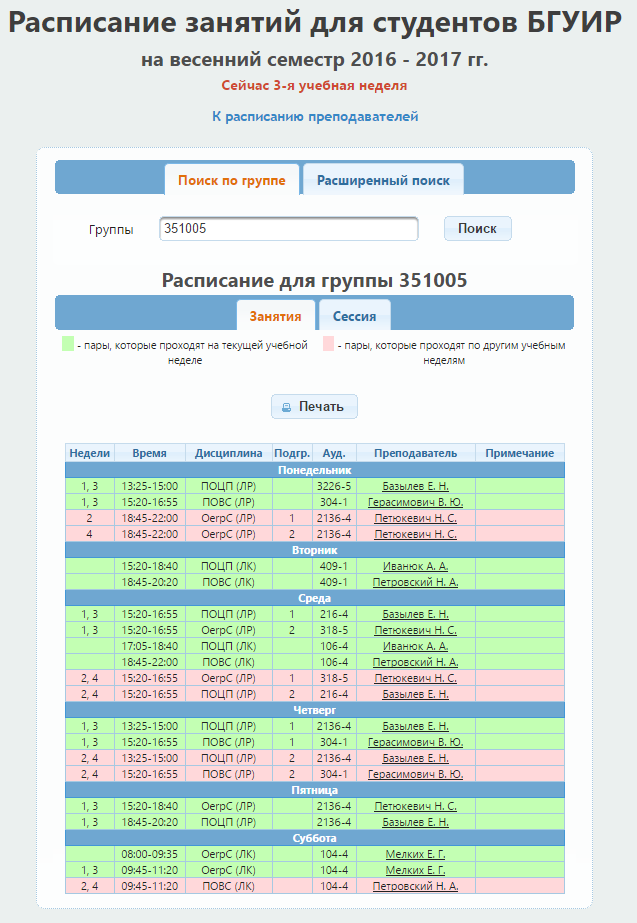
\includegraphics[scale=1]{schedule_bsuir_351005.png} 
	\caption{Пример расписания БГУИР}
	\label{fig:analysis:analogues:bsuir}
\end{figure}

\begin{figure}
	\centering
	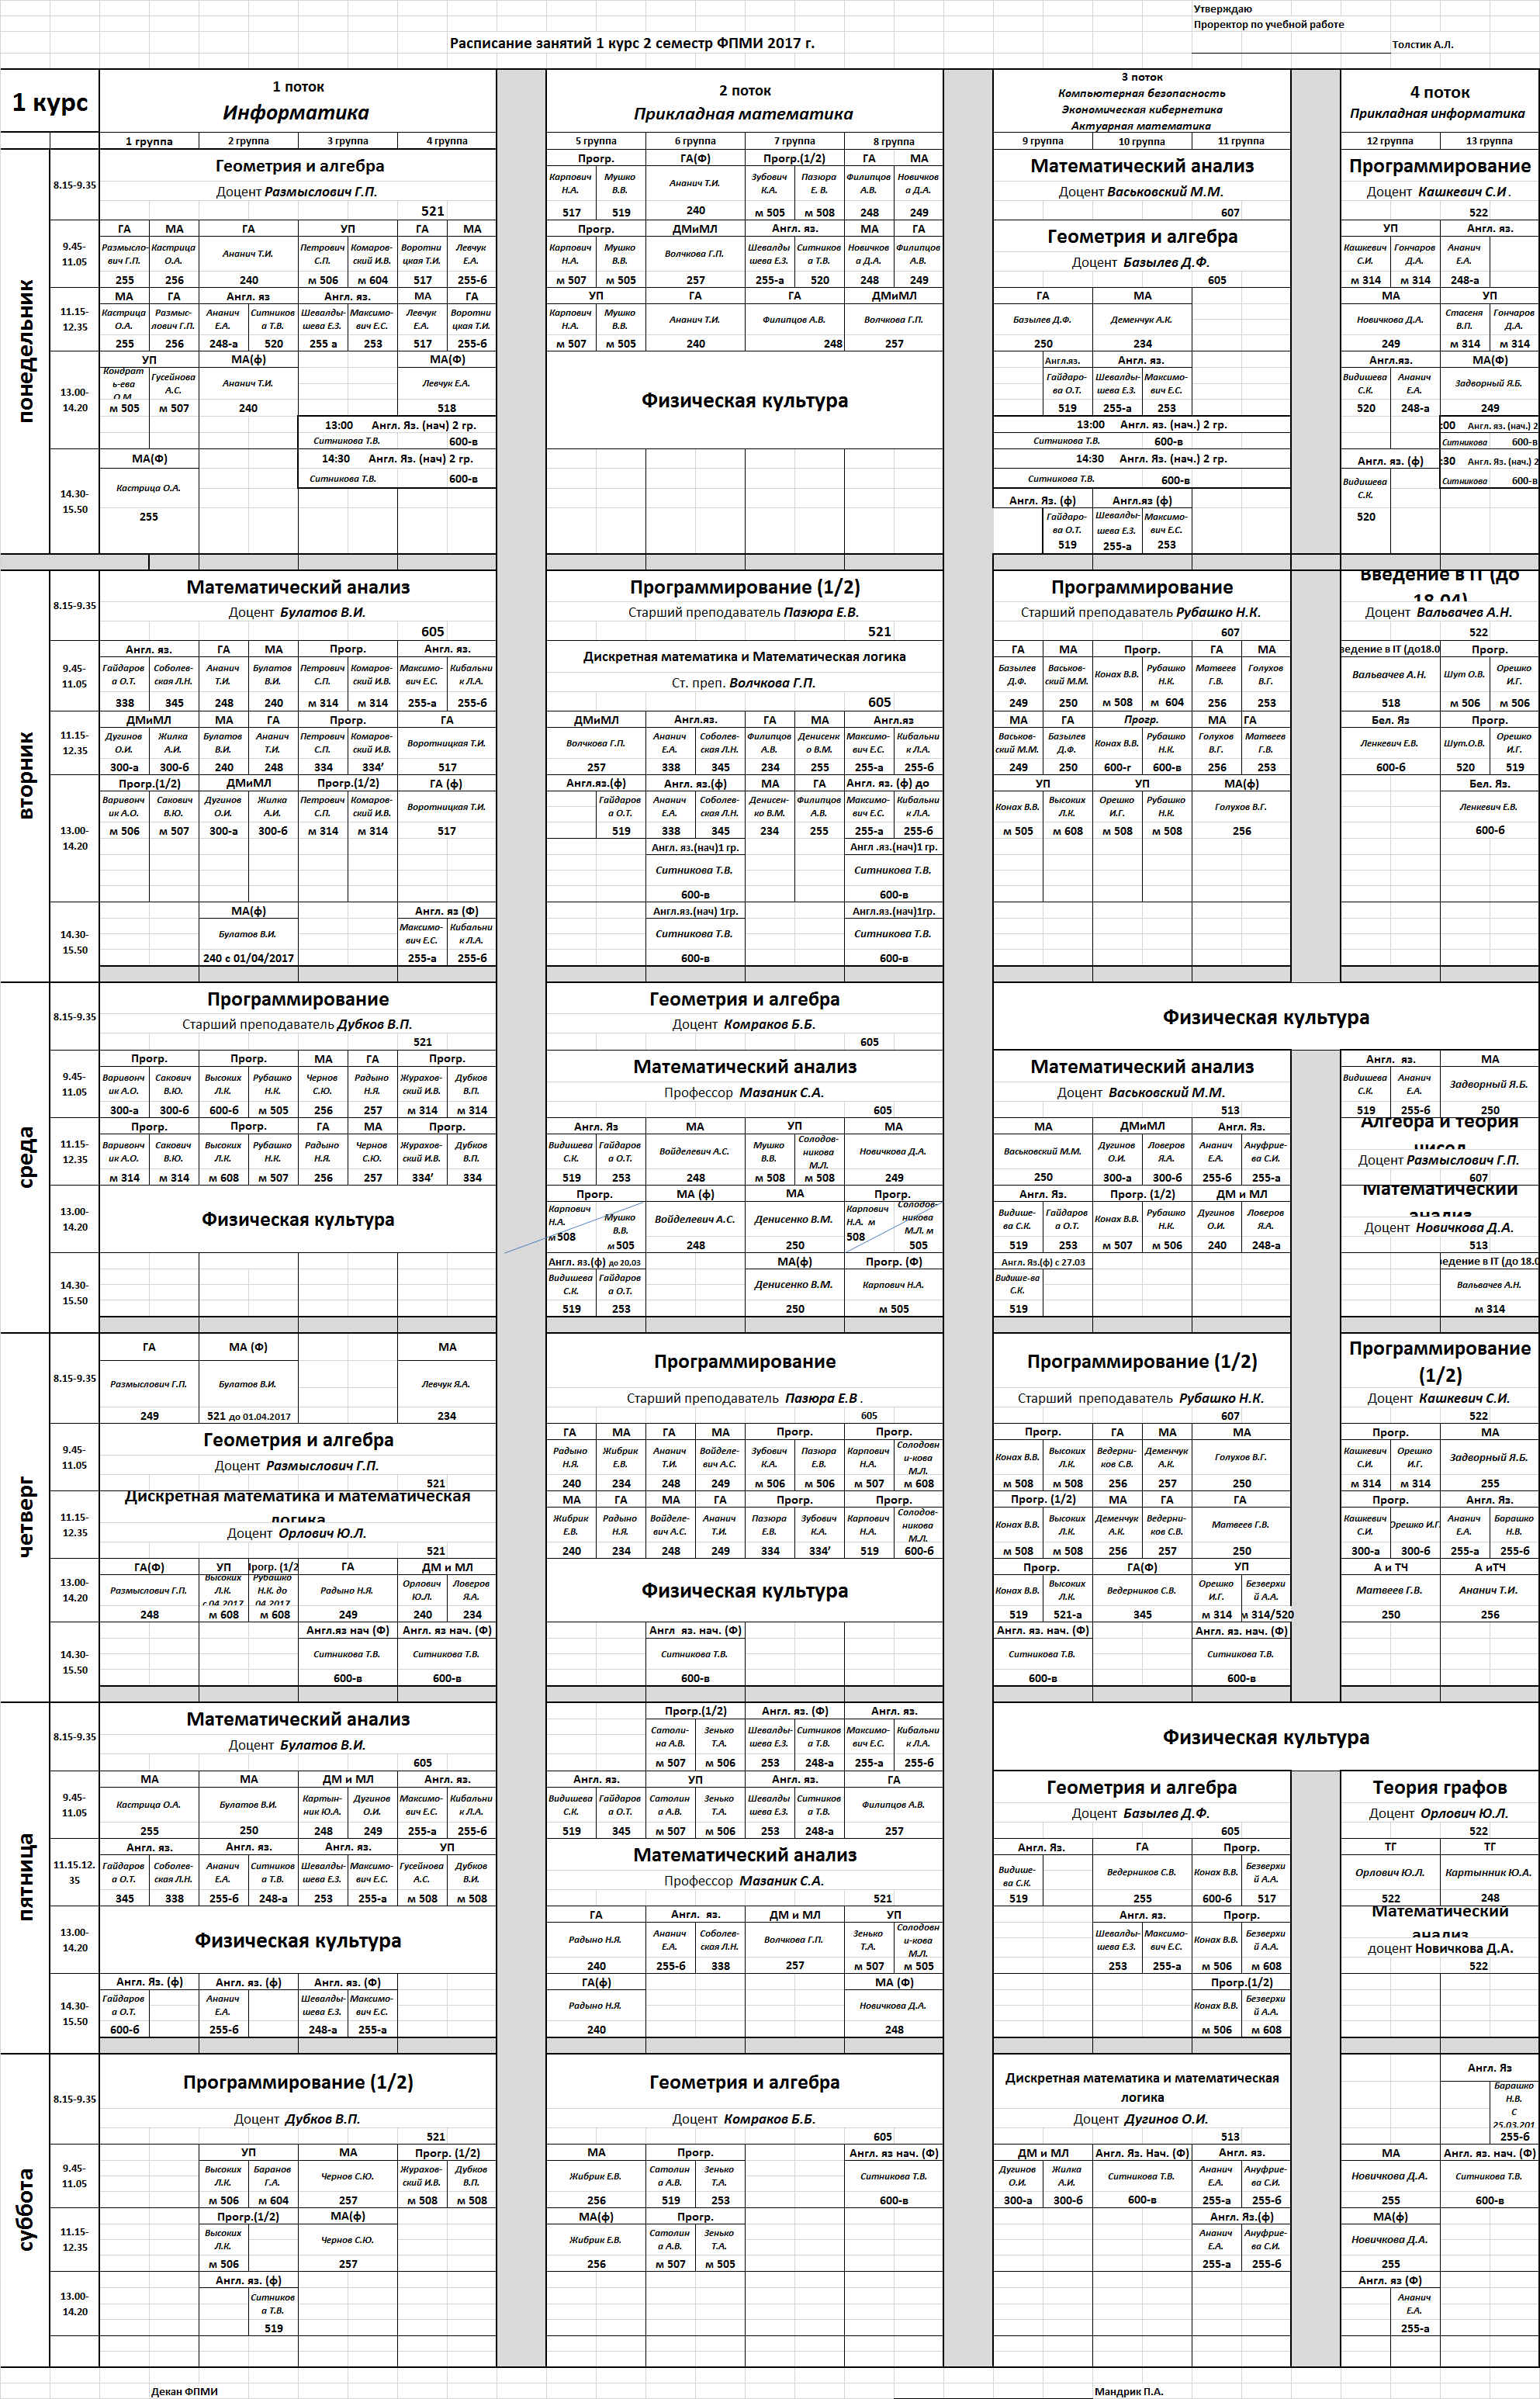
\includegraphics[scale=0.305]{schedule_bsu_fpmi_1kurs.png}
	\caption{Пример расписания ФПМИ БГУ}
	\label{fig:analysis:analogues:bsu_fpmi}
\end{figure}

Сайт ведущего университета страны общего профиля -- Белорусского государственного университета -- был значительно переработан около двух лет назад (то есть около февраля 2015 г.), что привело к значительному повышению удобства пользования и актуальности информации. Еще одним достоинством информационной системы БГУ является то, что для всех факультетов реализованы отдельные порталы. Однако, очень большим недостатком является то, что в этом университете не реализована единая система управления расписанием. Все факультеты решают задачу составления расписания и доставки его студентам и преподавателям по-своему. Есть факультеты, которые предоставляют более-менее удобные таблицы с расписанием (например, на рисунке \ref{fig:analysis:analogues:bsu_fpmi} приведен пример расписания первого курса ФПМИ), есть факультеты, которые предоставляют мобильное приложение с расписанием (но только с расписанием этого факультета), однако, есть факультеты, которые предоставляют расписание в виде неизменяемого и недоступного для автоматизированного разбора документа (например, в формате PDF). Более того, некоторые кафедры вообще не выкладывают своё расписание на сайт факультета, и чтобы студенты и преподаватели могли с ним ознакомиться, им нужно приходить к доске объявлений своей кафедры. В итоге, нет ни программного интерфейса для доступа к расписанию, ни даже унифицированной системы расписания, что значительно затрудняет создание любых приложений для работы с ним. И эту проблему в данном ВУЗе можно решить только одним способом: предложить систему, форматы данных и программные интерфейсы и каким-либо образом убедить их использовать. Но процесс информатизации не стоит на месте, и стоит ожидать, что уже скоро такая унификация произойдёт.

Попытка нивелировать неудобства пользования официальными источниками расписания может состоять в использовании специализированных сер\-висов-календарей. Как и все веб-приложения, они доступны на любом компьютере, подключенном к сети интернет, кроме того, зачастую разработаны официальные приложения для мобильных устройств. Еще одним достоинство является универсальность, заключающаяся в том, что данные сервисы можно использовать не только для управления занятиями университета. Главным же недостатком является необходимость вручную заполнять все расписание (что, однако, даёт возможность самому настроить форму его отображения). Таким образом, на конфигурирование таких приложений может уходить несколько часов пару раз в год. Пример расписания, сформированного с помощью веб-сервиса Google Calendar приведен на рисунке \ref{fig:analysis:analogues:google_calendar}. 

\begin{figure}[!h]
	\centering
	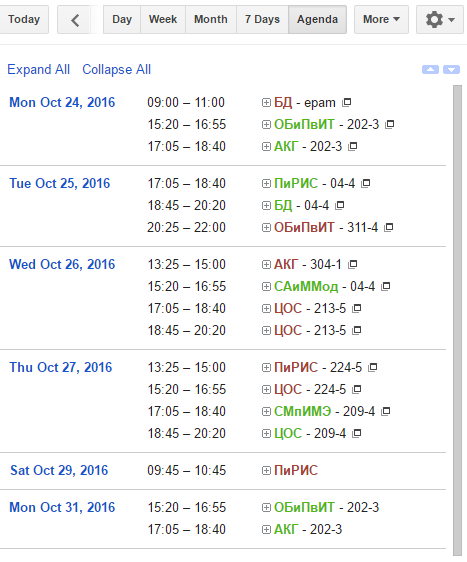
\includegraphics[scale=1]{google_calendar_agenda.png} 
	\caption{Пример расписания, сформированного с помощью сервиса Google Calendar}
	\label{fig:analysis:analogues:google_calendar}
\end{figure}

Анализ существующих информационных систем показывает наличие\linebreakразрозненности, отсутствие единого протокола обмена и хранения данных уче\-б\-но\-го процесса, что подтверждает актуальность разработки программного обе\-с\-пе\-че\-ния, направленного на автоматизацию данной области.

\subsubsection{} Управление задачами
\label{sec:analysis:analogues:tasks}

Управление задачами заключается в их учете и ранжированию по приоритету. Для этого могут использоваться различные записные книги и календари.

Самым первым средством стали обычные бумажные записные книги. И по сей день есть большое число их сторонников, для которых оказывается намного более удобным записать какие-то идеи на бумаге, чем в приложении на мобильном устройстве или компьютере \cite{paper_notebooks_power}. Из преимуществ выделяют следующие:

\begin{itemize}
	\item доступность, которая заключается в привычке постоянно держать бло\-к\-нот около себя;
	\item надежность, которая обусловлена независимостью от сети интернет и источников питания;
	\item визуализация и фиксация мыслей на бумаге часто помогает лучше обдумать задачу;
	\item универсальность: блокнот можно использовать и для записей, и для рисования, и для ведения адресной книги.
\end{itemize}

Тем не менее, следующие существенные недостатки данного способа влияют на выбор людей в пользу автоматизированных сервисов:

\begin{itemize}
	\item трудность внесения информации;
	\item высокая стоимость на единицу информации;
	\item сложность организации быстрого поиска.
\end{itemize}

Следующей альтернативой является использование приложений, эмулирующих записные книжки на компьютерах и мобильных устройствах. Таким приложений создано большое количество, многие из них обладают некоторыми отличительными чертами. Например, существуют приложения, которые позволяют приклеивать заметки к некоторым областям экрана (так называемые sticky notes). Зачастую приложения записных книг предлагают удобные способы разграничения заметок по цели их создания, например: заметки для работы, списки покупок и так далее. Кроме того, большинство приложений предоставляет возможность прикрепления различных видов информации к заметке: автосоздаваемые списки, таблицы, изображения, фотографии с камеры, звуковые заметки. 

\subsubsection{} Управление контактами
\label{sec:analysis:analogues:contacts}

Задача сохранения контактов актуальна и для студентов, поскольку они за время учебы взаимодействуют с несколькими десятками преподавателей, и, в свою очередь, для преподавателей, поскольку только за один семестр они сталкиваются с несколькими сотнями студентов. Проблема обеспечения двусторонней связи между ними актуальна в связи с существованием следующих задач:

\begin{itemize}
	\item проведение неформальных дистанционных консультаций;
	\item распространение индивидуальных заданий;
	\item распространение информации об изменениях в расписании.
\end{itemize}

В настоящее время для связи и сохранения контактов используются электронная почта и социальные сети. Электронная почта является стандартным средством коммуникации; практически все имеют хотя бы один зарегистрированный email. Тем не менее, слабая поддержка интерактивности и малый охват студентов сообщениями являются значительными недостатками данного средства. Частично данные недостатки решаются с помощью социальных сетей: там есть возможность создания круга контактов, есть возможность обмена мгновенными сообщениями и оповещения об изменениях большого количества людей. Однако, многие преподаватели уклоняются от пользования ими, по большей части из-за их развлекательной направленности. Чтобы исключить данный недостаток предлагается реализация социальной сети, ориентированной и специализируемой на учебном процессе.

\subsubsection{} Обзор некоторых средств дистанционного обучения
\label{sec:analysis:analogues:mooc}

Рассмотренные аспекты типичны для учебного процесса. При анализе возможностей их информатизации может возникнуть желание полностью оцифровать учебный процесс и осуществить полный переход к дистанционному обучению (или, по крайней мере, внедрить его наряду с другими формами обучения: очным и заочным). 

Дистанционная форма обучения в настоящее время осваивается различными университетами нашей страны, например, БГУИР, БГУ. Кроме того, существует большое число онлайн-ресурсов, предоставляющих доступ к обучающим курсам; наиболее известными из них являются Stanford Online, Coursera, Udacity, Khan Academy. Часто их объединяют под названием массовые открытые онлайн-курсы (MOOC -- massive open online courses~\cite{mooc_model}). 

В настоящее время практически любое учебное заведение может создать свой онлайн-ресурс дистанционного обучения. Для этого может применяться одна из специальных программных систем, наиболее известной и распространенной из которых является свободная система управления курсами Moodle. Данная система разрабатывается сотрудниками специального фонда, который финансируется партнерами системы и грантами. Основная функциональность доступна в стандартной поставке, также есть возможность установки сторонних модулей (необязательно бесплатных). На рисунках~\ref{fig:analysis:analogues:moodle_home},~\ref{fig:analysis:analogues:moodle_calendar},~\ref{fig:analysis:analogues:moodle_course_home} приведены примеры экранов развернутой и функционирующей системы Moodle.

\begin{figure}
\centering
	\begin{subfigure}[ht]{0.85\textwidth}
	    \centering
		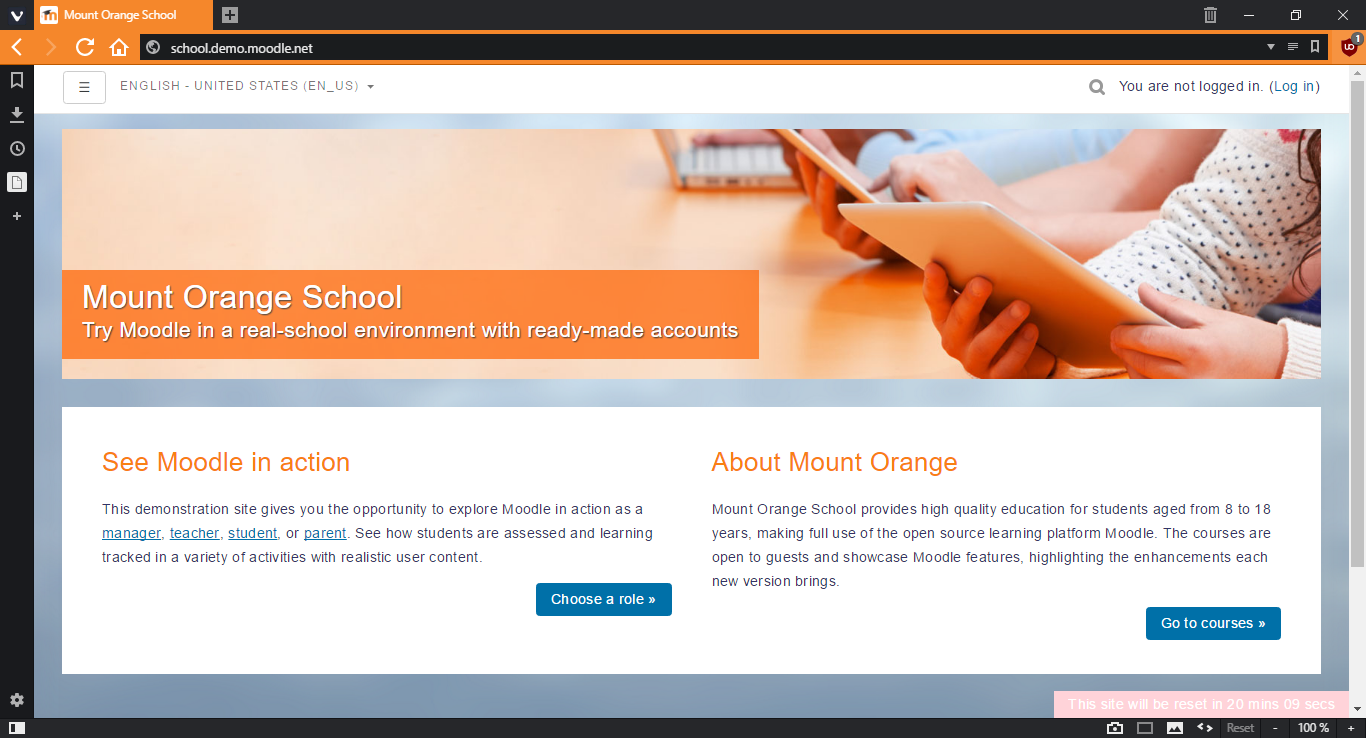
\includegraphics[width=1\linewidth]{moodle_home.png}
		\caption{домашняя страница системы Moodle}
		\label{fig:analysis:analogues:moodle_home}
	\end{subfigure}
	\begin{subfigure}[ht]{0.85\textwidth}
	    \centering
		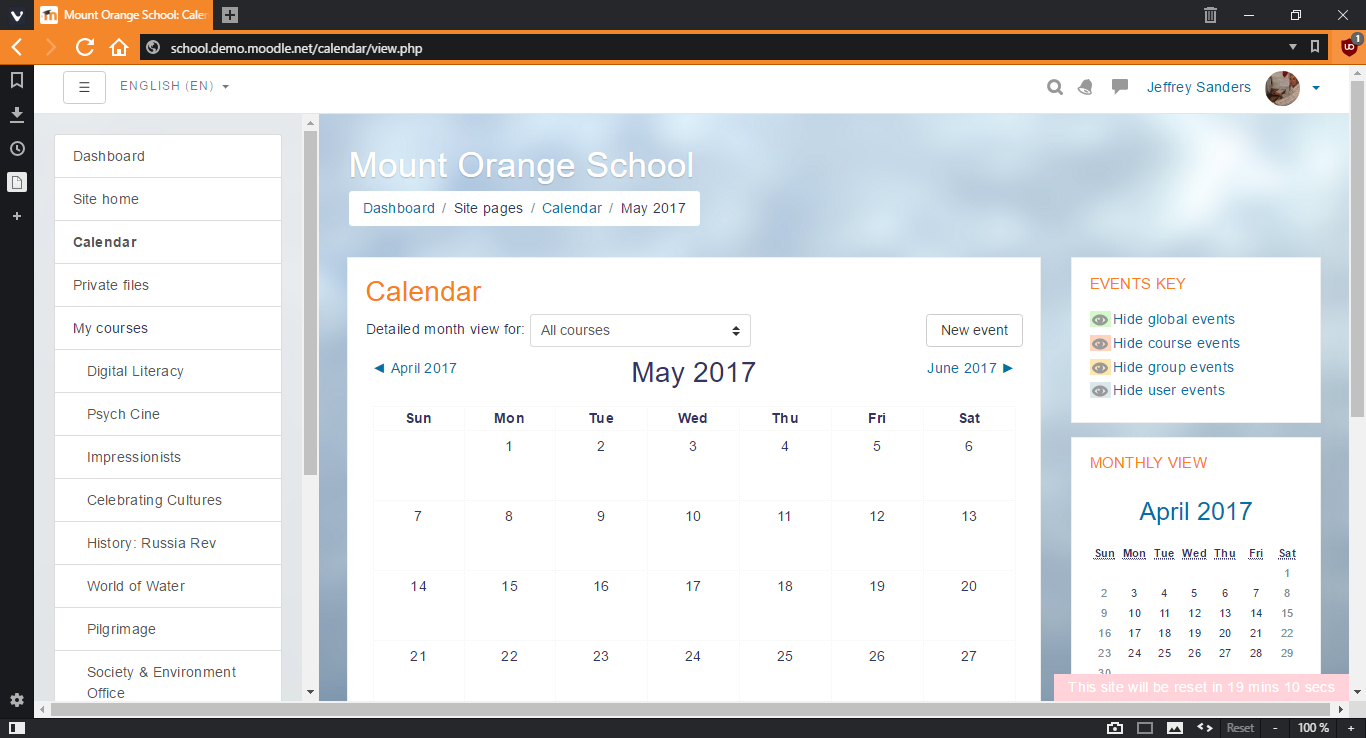
\includegraphics[width=1\linewidth]{moodle_calendar.png}
		\caption{экран календаря Moodle}
		\label{fig:analysis:analogues:moodle_calendar}
	\end{subfigure}
	\begin{subfigure}[ht]{0.85\textwidth}
	    \centering
		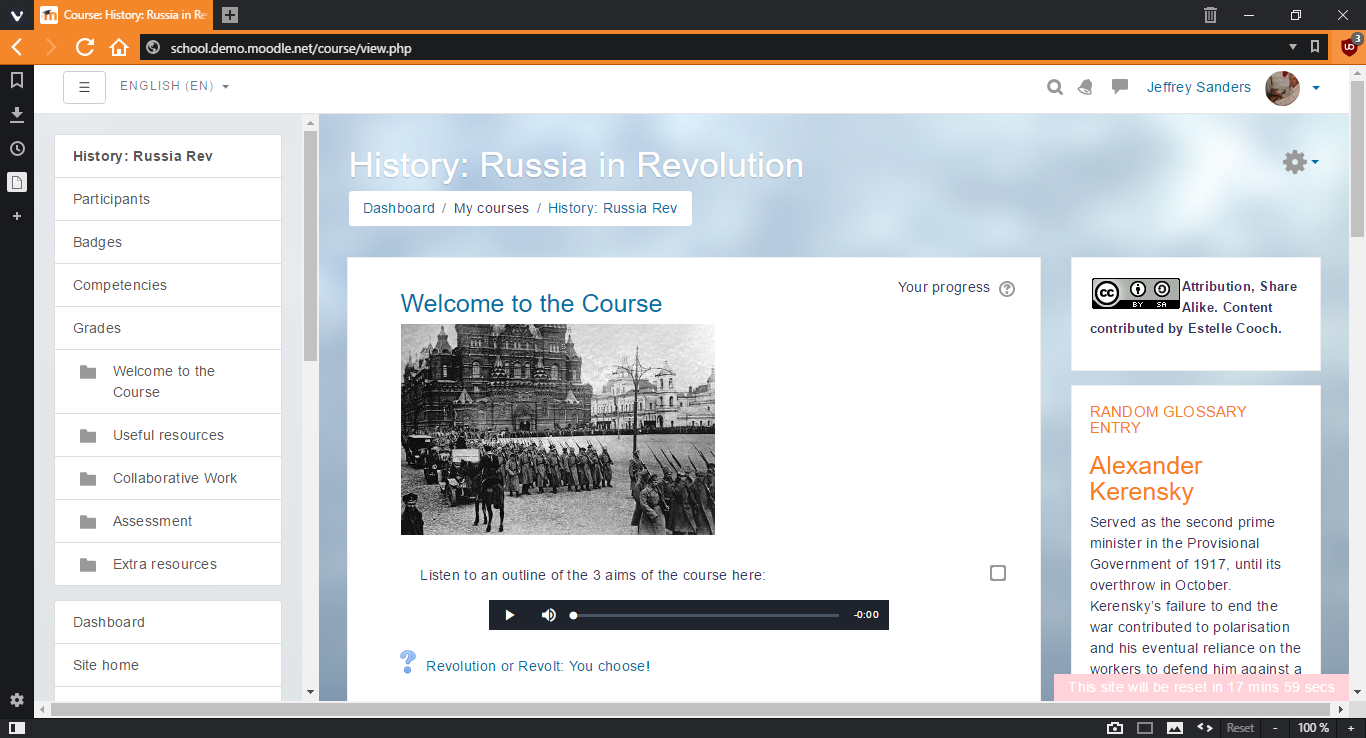
\includegraphics[width=1\linewidth]{moodle_course_home.png} 
		\caption{экран домашней страницы курса Moodle}
		\label{fig:analysis:analogues:moodle_course_home}
	\end{subfigure}
	\caption{Примеры экранов системы Moodle}
\end{figure}

Система Moodle разрабатывается с 2002 года~\cite{moodle_habr}, она обладает достаточной стабильностью, кроме того, процесс её установки автоматизирован с помощью специального мастера. Тем не менее, если сравнивать предложенные в ней концепции с проектируемой в данном дипломном проекте программной системой, то существенными оказываются следующие вопросы:
\begin{itemize}
	\item Система Moodle является решением для дистанционного обучения. Конечно, ее применение возможно и для других форм, однако это не является целью её разработки, а побочной возможностью.
	\item Данная система требует нового развертывания и инстанциирования у каждого нового заказчика, то есть предполагается архитектурный стиль множественности экземпляров программного средства (multiinstance). При его применении требуется наличие специалистов поддержки у каждого заказчика. Кроме того, большое число экземпляров системы лишает возможности экономии вычислительных мощностей и средств хранения. Для решения данной проблемы планируется использование мультиарендного архитектурного стиля (mul\-ti\-te\-nan\-cy), когда создается единый экземпляр приложения, который обслуживает множество заказчиков (в нашем случае -- множество \mbox{ВУЗов}).
	\item Сложность пользования системой в связи с запутанностью интерфейса. Разработчики реализовали достаточно большой набор функциональности, который, однако, не обладает свойством удобства пользования. О данном факте свидетельствуют многочисленные отзывы студентов и преподавателей университетов, в которых была внедрена данная система~\cite{moodle_habr}.
\end{itemize}

Все озвученные системы дистанционного обучения относятся к предметной области обучения студентов. Значит, и их проектирование и разработка начиналась и отталкивалась от анализа очной формы обучения. Таким образом решалась задача переноса взаимодействия участников учебного процесса в онлайн-среду. Однако целью данного дипломного проекта является не разработка системы для дистанционного обучения, а привнесение их положительных средств и свойств в очное образование с единственной целью -- облегчения некоторых задач участников учебного процесса.
